% Report for YAMS, project in CWRU EECS 314 Spring 2015
%
% Members:
%    Stephen Brennan (smb196)
%    Katherine Cass (krc53)
%    Jeffrey Copeland (jpc86)
%    Andrew Mason (ajm188)
%    Thomas Murphy (trm70)
%    Aaron Neyer (agn31)

\documentclass[journal,10pt]{IEEEtran}
% Will correctly load from ./
% Explicit use of 10pt by report requirements

% *** GRAPHICS RELATED PACKAGES ***
%
\ifCLASSINFOpdf
 \usepackage[pdftex]{graphicx}
\else
 \usepackage[dvips]{graphicx}
\fi

% declare the path(s) where your graphic files are
\graphicspath{{screenshots/}}
% declare graphics file extensions
\DeclareGraphicsExtensions{.pdf,.jpeg,.png}

% *** MATH PACKAGES ***
%
\usepackage[cmex10]{amsmath}

% *** PDF, URL AND HYPERLINK PACKAGES ***
%
\usepackage{url}
% url.sty was written by Donald Arseneau. It provides better support for
% handling and breaking URLs.
% Basically, \url{my_url_here}.

% Correctly create hyperlinks with URLs
\usepackage{hyperref}

% Allow nicer float options
\usepackage{float}

% correct bad hyphenation here
\hyphenation{op-tical net-works semi-conduc-tor}


\begin{document}
% paper title
\title{YAMS: Awesome MIPS Server}

% author names
\author{
Stephen~Brennan,
Katherine~Cass,
Jeffrey~Copeland,
Andrew~Mason,
Thomas~Murphy,
Aaron~Neyer% stop_space
\thanks{All authors are with the Department of Electrical Engineering and Computer Science, Case Western Reserve University, Cleveland, OH, 44106 USA}% stop_space
\thanks{Final Report submitted May 1, 2015, typographical revisions and clarifications May 28, 2015.}
} % Close the author environment


% The paper headers
\markboth{CWRU EECS 314 Spring 2015 Final Project}%
{}
% The only time the second header will appear is for the odd numbered pages
% after the title page when using the twoside option.

% make the title area
\maketitle

% As a general rule, do not put math, special symbols or citations
% in the abstract or keywords.
\begin{abstract}
We set out to build a simple web server in MIPS. Mission Accomplished.
\end{abstract}

% Note that keywords are not normally used for peerreview papers.
\begin{IEEEkeywords}
MIPS, computer architecture, HTTP, server, MARS, ISA simulation.
\end{IEEEkeywords}

% Begin body of the report

\section{Problem Statement}

\IEEEPARstart{T}{he} goal of this project was to write a static HTTP server in
MIPS assembly running in the MARS simulator. The server would be able to serve a
website, which is contained in the \texttt{html/} directory on port 19001. The
content would then be viewable in a browser. Sockets would be used for
networking and implemented in extending MARS syscalls, making the high-level
networking features accessible from simulated MIPS assembly.


\section{Major Challenges}

The first major challenge in YAMS was implementing socket syscalls. MARS was
chosen early on because it allowed for custom syscalls; however, we only found
sparse documentation. This required us to learn about MARS through trial and
error. Additionally, if one stops MARS while waiting on a socket syscall, the
simulator enters an error state, forcing us to either 1) double-reassemble-run
the program, or 2) restart all of MARS. These additional steps made debugging
much slower than simulating a program without the unexpected behavior of the
Java/MARS sockets.

The larger challenge in implementing YAMS was parsing HTTP requests. RFC
2616\cite{Leach}, our HTTP (Hypertext Transfer Protocol) reference for this
project, is 175 pages long. While it is possible to implement a full HTTP stack
in assembly, it is difficult to do in one or two months. Thus, we focused on
what was required to get web pages to display in a browser: GET, POST, Expect,
and only identity encoding or Content-Length. Additionally, because the request
parser had to interact with the socket differently depending on the request
header (e.g. Transfer-Encoding, Content-Length, and Expect), our testing and
debugging revolved around trial-and-error requests with the Unix program
\texttt{curl} and browsers.

\section{System Components}

After submission of the report, the entirety of the implementation is available at \cite{Brennan}. The breakdown of the system components is as follows.

\subsection{String Operations}

In order to parse HTTP requests, we needed to implement much of the C standard
string library. In \texttt{mips/string.asm}, we implemented \texttt{strlen},
\texttt{strncpy}, \texttt{memcpy}, \texttt{strcmp}, \texttt{strncmp},
\texttt{atoi}, \texttt{htoi}, \texttt{strcat}, \texttt{strncat}, as well as two
functions for identifying the index of characters and substrings,
\texttt{str\_index\_of} and \texttt{substr\_index\_of} respectively. To verify
their correctness, we wrote tests in \texttt{mips/test\_string.asm}. They can
be run in MARS by loading that file as the main file, instead of
\texttt{mips/main.asm}.

\subsection{HTTP Request Handling}

As mentioned in Major Challenges, our focus with request parsing was on serving
a page that a browser could render. Therefore, we chose to support a subset of
HTTP request statuses (e.g. GET, POST), look for a few headers (e.g.
Content-Length, Expect), and read or write through the socket accordingly. The
logic for request parsing is in \texttt{http-requests.asm}, and is reached
through the \texttt{get\_request} method from \texttt{main}, returning an
internal HTTP request type, and, as applicable, request URI, request body,
request body length, and content type. The main method takes this data and
hands it off to the file loader and response builder.

The request parser functionality was validated through trial-and-error: seeing
if debug prints contained the right information and if the browser loaded the
page properly. The mixture of MIPS assembly and MARS syscall extensions
precluded the use of unit tests to verify the correctness of the parser's
behavior in the given time.

\subsection{File Access}

File access is already implemented in the MARS default syscalls, saving us the
trouble of adding this feature to the simulator. These calls were wrapped in
function-like macros for ease of use.

Additionally, the HTTP handling receives URIs (uniform resource identifiers),
not system paths. These strings needed processing to produce a valid file path
that could be consumed by the MARS syscall. Our processing, implemented in
\texttt{mips/file.asm}, is composed of substring-blacklisting to prevent the
\texttt{../} directory from being used to access arbitrary system resources and
string operations to modify the URI into a useful file path. The file path is
created using the default \texttt{html/} directory (where our web resources are
stored) as the base relative file path and URIs with a trailing \texttt{/} have
the file name \texttt{index.html} appended. The processing operation has tests
implemented in \texttt{mips/test\_file.asm}.

\subsection{Turing Tape Language Interpreter}

As an additional stretch feature, we implemented an interpreter for the
esoteric programming language Brainfuck\cite{Mpreu/preller}. This simple
language simulates a Turing machine's operations and has only 8 commands (each
of which is a single character). The interpreter is implemented in
\texttt{mips/brainfuck.asm}, and tested in \texttt{mips/test\_brainfuck.asm}.
When the server is running, code can be loaded into the interpreter by sending a
POST request to the URL \texttt{/load}. The code can then be run by sending
input in a POST request to the URL \texttt{/run}, which will return the program
output in its response. For a more accessible interface, the URL
\texttt{/brainfuck.html} provides a simple page that uses JavaScript to transfer
the code and input to the interpreter and receive the resultant output.

\section{Component Integration}

In order to integrate these different components into a cohesive project, we had
to define and follow a strict calling convention. We decided that all functions
would be called using the \texttt{JAL} instruction. Only the \texttt{\$s0-\$s7}
saved registers and global pointers would be preserved across function calls.
Arguments were passed (and not necessarily preserved) in the \texttt{\$a0-\$a3}
registers and return values were placed in the \texttt{\$v0-\$v1} registers. Any
additional arguments or return values would be placed on the stack. It was the
caller's responsibility to push the return address of its scope and any other
registers which it wanted preserved to the stack prior to calling the next
function. To facilitate conforming to these rules, we defined macros in
\texttt{mips/util-macros.asm} for pushing to and popping from the stack to make
those operations semantically clear in our code.

\section{User Interface}

We have implemented an HTTP server, so the functional interface is through a web
socket while the debug interface is the standard output of the MARS simulator.
To compile MARS with our implemented syscalls, run \texttt{make} from the
project root. Then run \texttt{java -jar Mars4\_5-SockMod.jar} or directly open
the JAR to use the modified version of MARS. Load the \texttt{mips/main.asm}
file into the simulator. Assemble and run that to start a server listening on
port 19001 (\texttt{\url{http://localhost:19001/}}). Now, the content in the
\texttt{html/} directory is hosted at the root of the server. The content we
created for this project is rendered below as our interface examples.
Alternatively, the server can be accessed using the Unix tool \texttt{curl}.

\section{Documentation of Runs}

\subsection{Static Page Content}

The static page in Fig.~\ref{fig:static_document} is hosted as the
\texttt{/index.html} document of the server. This is the document the user would
expect to load into their browser upon access to the root page of the server.
This demonstrates the ability to serve multiple resources for a page: images,
fonts, and the HTML.

\subsection{Dynamic JavaScript Content}

The dynamic page in Fig.~\ref{fig:dynamic_document} is the presentation given to
the class on April 23, 2015. This document uses HTML, JavaScript, and images.
All resources are loaded from YAMS and not from external internet hosts.

\subsection{Interactive AJAX Content}

The final dynamic-content page, shown in Fig.~\ref{fig:interactive_ajax}, is the
front end interface for the YAMS server's Brainfuck\cite{Mpreu/preller}
interpreter. The page interacts with the interface through POST requests and
updates the text field on the page when it receives the result of running the
user-supplied Brainfuck code and input.

\section{Group Member Contributions}

\begin{LaTeXitemize} \itemsep0pt \parskip0pt
  \item Stephen Brennan
  \begin{enumerate}
    \item String functions
    \item Brainfuck interpreter
  \end{enumerate}

  \item Katherine Cass
  \begin{enumerate}
    \item Static site
    \item Report content
  \end{enumerate}

  \item Jeffrey Copeland
  \begin{enumerate}
    \item Socket syscalls
    \item HTTP request handling
  \end{enumerate}

  \item Andrew Mason
  \begin{enumerate}
    \item HTTP response building
    \item Project presentation
  \end{enumerate}

  \item Thomas Murphy
  \begin{enumerate}
    \item File access
    \item Code formatting and style
    \item Report organization and typesetting
  \end{enumerate}

\end{LaTeXitemize}

Aaron Neyer planned to build a website documenting our project, but could not
complete it due to personal circumstances.

\section{Conclusion}

We started this project to build a simple web server in MIPS. Despite the high
upfront workload, our collective components merged into what has been called ``a
surprsingly robust web server.'' Thus, we have achieved our goal: writing a
static webserver in MIPS and MARS.

\appendices

\onecolumn % use single column for the wide columns
\section{Screenshots of Code Execution Results}

\begin{figure}[H]
\centering
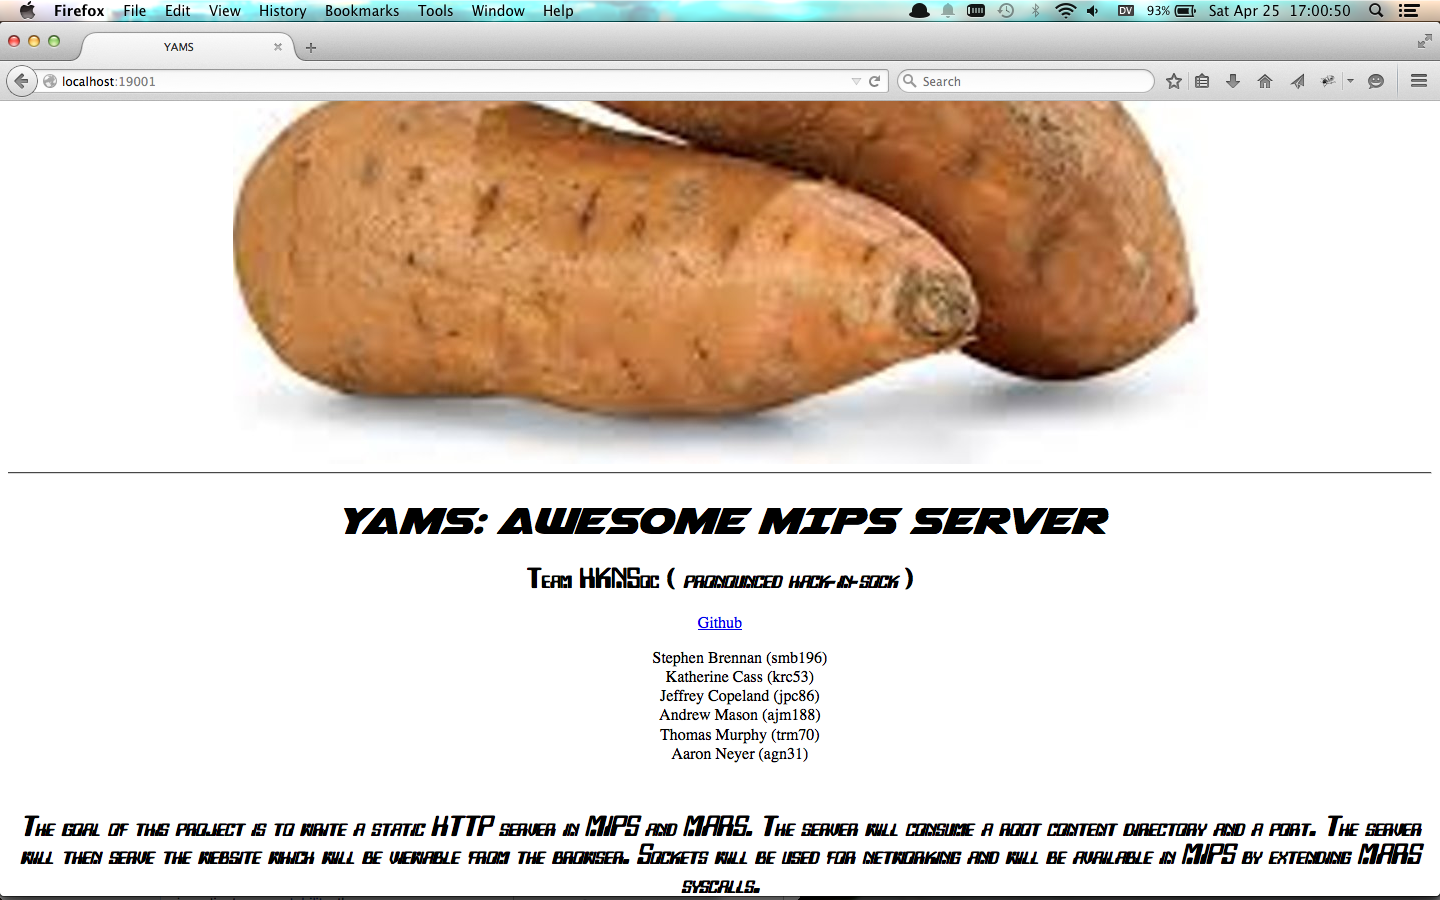
\includegraphics[width=0.8\textwidth,natwidth=1440,natheight=900]{static_document}
\caption{The static \texttt{index.html} served by YAMS by default.}
\label{fig:static_document}
\end{figure}

\begin{figure}[H]
\centering
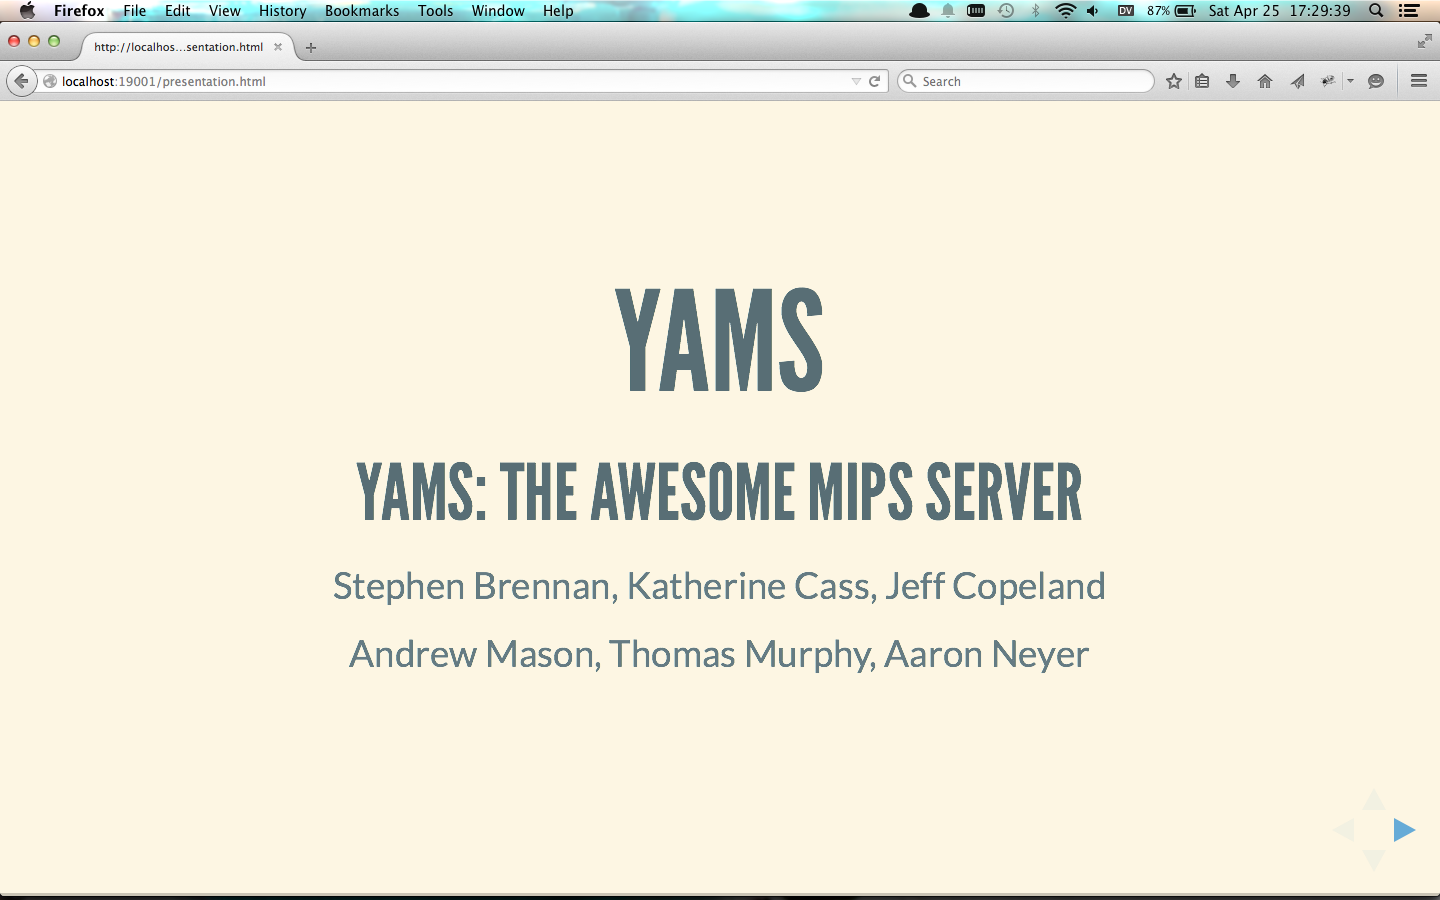
\includegraphics[width=0.8\textwidth,natwidth=1440,natheight=900]{dynamic_document}
\caption{The first view of a dynamic HTML/JavaScript page containing the material presented to the class.}
\label{fig:dynamic_document}
\end{figure}

\begin{figure}[H]
\centering
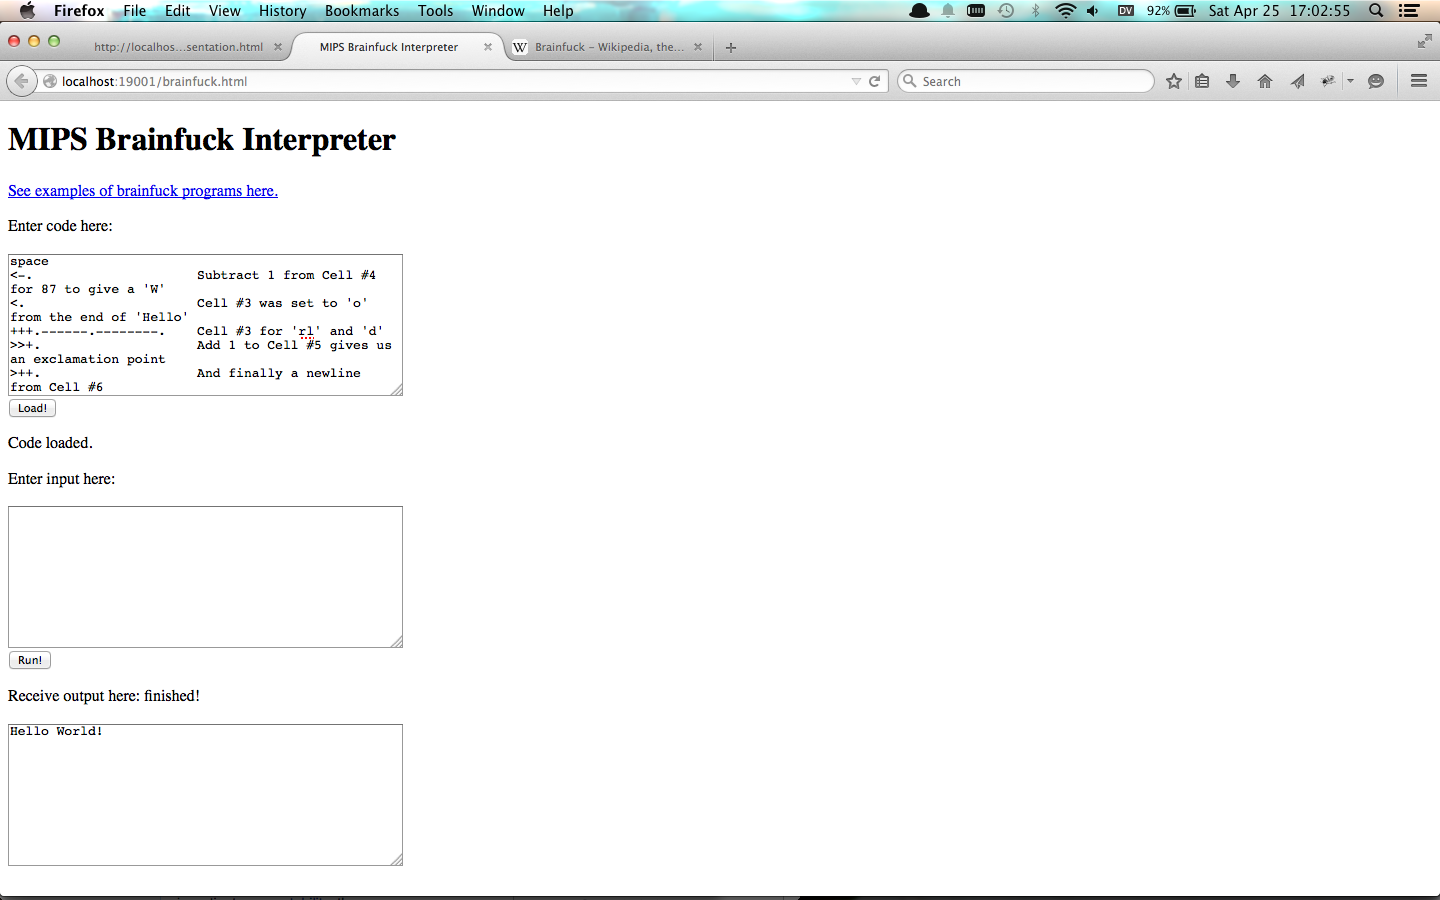
\includegraphics[width=0.8\textwidth,natwidth=1440,natheight=900]{interactive_ajax}
\caption{A web interface to an implementation of the Brainfuck interpreter contained within YAMS.}
\label{fig:interactive_ajax}
\end{figure}

\twocolumn % return to two columns

% use section* for acknowledgment
\section*{Acknowledgment}


The authors would like to thank Cameron Gutman
(\texttt{\url{https://github.com/cgutman}}) for providing information about the
usage of identity transfer encoding.

% references section
\bibliography{IEEEabrv,./yams_report}
\bibliographystyle{IEEEtran}
\nocite{*}

% that's all folks
\end{document}
